\documentclass[11pt]{article}

\usepackage[margin=1in]{geometry}
\usepackage{amsmath, amssymb, amsthm}
\usepackage{tikz}
\usetikzlibrary{positioning, arrows.meta, fit, backgrounds, calc}
\usepackage{hyperref}

\title{Learning Embeddings for a Pursuit--Evasion Differential Game}
\author{}
\date{}

\begin{document}
\maketitle

\section{Game setup}

We consider a two-player pursuit--evasion differential game between an
\emph{evader} $E$ and a \emph{pursuer} $P$ in the plane.
Each agent's velocity is decomposed into a (fixed) magnitude and a unit
direction:
\begin{equation}
  \vec{v} \;=\; \|\vec{v}\| \cdot \hat{u},
  \qquad \hat{u} \in \mathbb{S}^{1}.
\end{equation}

The speeds are fixed hyperparameters of the game,
\begin{equation}
  v_E \;=\; \text{fixed}, \qquad v_P \;=\; \text{fixed},
\end{equation}
and, without loss of generality, the pursuer starts at the origin:
\begin{equation}
  \vec{x}_P(0) \;=\; (0,\,0).
\end{equation}

The state of the game at time $t$ is the pair of positions
$\bigl(\vec{x}_E(t),\,\vec{x}_P(t)\bigr) \in \mathbb{R}^2 \times \mathbb{R}^2$,
evolving on the interval $t \in [0, t_{\max}]$ according to
\begin{equation}
  \dot{\vec{x}}_E(t) \;=\; \vec{v}_E(t), \qquad
  \dot{\vec{x}}_P(t) \;=\; \vec{v}_P(t).
\end{equation}

\section{Neural network embeddings}

Each agent has its own neural network that, at every time $t$, embeds the
current game state into a \emph{unit direction} of motion.  Writing the
network outputs as $\hat{u}_E^{NN}$ and $\hat{u}_P^{NN}$, the actual
velocities used to advance the dynamics are obtained by rescaling these
embeddings by the (fixed) speeds:
\begin{align}
  \vec{v}_E(t) &\;=\; \|\vec{v}_E\| \cdot \hat{u}_E^{NN}\!\bigl(\vec{x}_E(t),\,\vec{x}_P(t)\bigr), \\
  \vec{v}_P(t) &\;=\; \|\vec{v}_P\| \cdot \hat{u}_P^{NN}\!\bigl(\vec{x}_E(t),\,\vec{x}_P(t)\bigr).
\end{align}

The two-network architecture (one per player) is depicted below.  The
inputs $x_{E,1}, x_{E,2}$ are the components of the evader's position and
$x_{P,1}, x_{P,2}$ are the components of the pursuer's position; the
outputs $\vec{v}_{E,1}(t), \vec{v}_{E,2}(t)$ and
$\vec{v}_{P,1}(t), \vec{v}_{P,2}(t)$ are the components of the resulting
velocity vectors.

\begin{center}
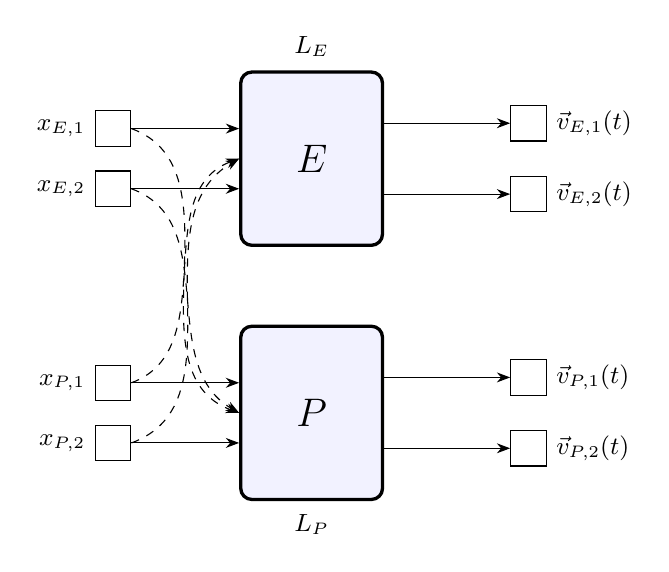
\begin{tikzpicture}[
    >=Stealth,
    node distance=1.2cm and 1.6cm,
    nn/.style={draw, very thick, rounded corners=4pt,
               minimum width=1.8cm, minimum height=2.2cm,
               font=\Large\bfseries, fill=blue!5},
    io/.style={draw, minimum width=0.45cm, minimum height=0.45cm,
               fill=white},
    every label/.style={font=\small}
]

%---------------- Evader sub-network ----------------
\node[io, label=left:$x_{E,1}$] (xE1) {};
\node[io, below=0.3cm of xE1, label=left:$x_{E,2}$] (xE2) {};

\node[nn, right=1.6cm of $(xE1)!0.5!(xE2)$] (E) {$E$};
\node[above=0.05cm of E, font=\small] {$L_E$};

\node[io, right=1.6cm of E, yshift=0.45cm,
      label=right:{$\vec{v}_{E,1}(t)$}] (vE1) {};
\node[io, right=1.6cm of E, yshift=-0.45cm,
      label=right:{$\vec{v}_{E,2}(t)$}] (vE2) {};

\draw[->] (xE1) -- (E.west |- xE1);
\draw[->] (xE2) -- (E.west |- xE2);
\draw[->] (E.east |- vE1) -- (vE1);
\draw[->] (E.east |- vE2) -- (vE2);

%---------------- Pursuer sub-network ----------------
\node[io, below=2.0cm of xE2, label=left:$x_{P,1}$] (xP1) {};
\node[io, below=0.3cm of xP1, label=left:$x_{P,2}$] (xP2) {};

\node[nn, right=1.6cm of $(xP1)!0.5!(xP2)$] (P) {$P$};
\node[below=0.05cm of P, font=\small] {$L_P$};

\node[io, right=1.6cm of P, yshift=0.45cm,
      label=right:{$\vec{v}_{P,1}(t)$}] (vP1) {};
\node[io, right=1.6cm of P, yshift=-0.45cm,
      label=right:{$\vec{v}_{P,2}(t)$}] (vP2) {};

\draw[->] (xP1) -- (P.west |- xP1);
\draw[->] (xP2) -- (P.west |- xP2);
\draw[->] (P.east |- vP1) -- (vP1);
\draw[->] (P.east |- vP2) -- (vP2);

%---------------- Cross-coupling (each net sees both positions) ----------------
\draw[->, dashed] (xP1.east) to[out=20, in=200] (E.west);
\draw[->, dashed] (xP2.east) to[out=20, in=210] (E.west);
\draw[->, dashed] (xE1.east) to[out=-20, in=160] (P.west);
\draw[->, dashed] (xE2.east) to[out=-20, in=150] (P.west);

\end{tikzpicture}
\end{center}

\noindent\textit{Solid arrows: an agent's own positions feed its network.
Dashed arrows: the opponent's positions are also provided as input, since
each policy depends on the relative configuration of the two players.}

\medskip

\noindent A more compact view of the same architecture treats each network
as a black box producing the player's velocity:
\begin{equation}
  \bigl(\vec{x}_E,\,\vec{v}_E^{NN},\,\vec{v}_P^{NN}\bigr)
  \;\longmapsto\;
  \bigl(\vec{v}_E(t),\, \vec{v}_P(t)\bigr).
\end{equation}

\section{Loss functions}

Let $\varepsilon > 0$ denote the capture radius and let
$t_{\max}$ be the time horizon of a rollout.
Define the capture condition
\begin{equation}
  \mathcal{C} \;:\;\;
  \exists\, T \le t_{\max} \;\text{such that}\;
  \|\vec{x}_E(T) - \vec{x}_P(T)\| \le \varepsilon,
  \qquad t \in [0, t_{\max}].
\end{equation}

\paragraph{Case 1 -- capture occurs at time $T$.}
The pursuer is rewarded for catching the evader as quickly as possible,
while the evader is penalised for being caught early:
\begin{equation}
  L_E \;\propto\; \frac{1}{T},
  \qquad
  L_P \;\propto\; T.
\end{equation}

\paragraph{Case 2 -- no capture within the horizon.}
If $\mathcal{C}$ does not hold, the loss falls back to the final
separation distance:
\begin{equation}
  L_E \;\propto\; \frac{1}{\|\vec{x}_E - \vec{x}_P\|},
  \qquad
  L_P \;\propto\; \|\vec{x}_E - \vec{x}_P\|.
\end{equation}

Summarising as a piecewise objective,
\begin{equation}
  L_E \;=\;
  \begin{cases}
    \dfrac{1}{T} & \text{if } \mathcal{C} \text{ holds at time } T, \\[6pt]
    \dfrac{1}{\|\vec{x}_E(t_{\max}) - \vec{x}_P(t_{\max})\|}
                 & \text{otherwise,}
  \end{cases}
  \qquad
  L_P \;=\;
  \begin{cases}
    T & \text{if } \mathcal{C} \text{ holds at time } T, \\
    \|\vec{x}_E(t_{\max}) - \vec{x}_P(t_{\max})\|
      & \text{otherwise.}
  \end{cases}
\end{equation}

The two networks are trained adversarially: gradients of $L_E$ update the
evader's parameters, gradients of $L_P$ update the pursuer's.  The unit
vectors $\hat{u}_E^{NN}, \hat{u}_P^{NN}$ produced by the networks act as
\emph{embeddings} of the current game state into the optimal direction
of motion under each player's objective.

\end{document}
